\subsubsection{Fase 1}
\mbox{\hspace{-6ex}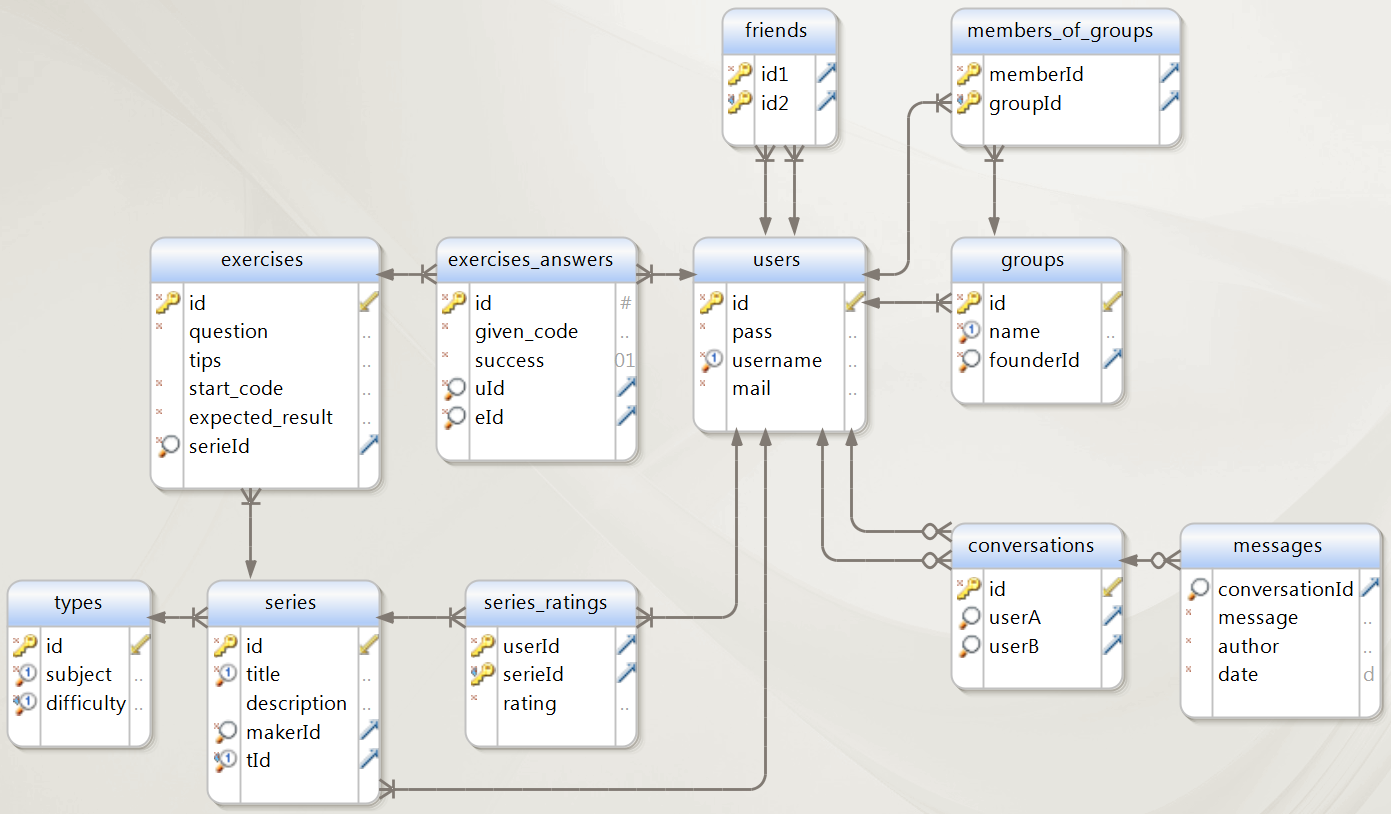
\includegraphics[keepaspectratio=true, scale=0.4]{raport_files/design/UML1.png}}
\subsubsection{Fase 2}
\mbox{\hspace{-6ex}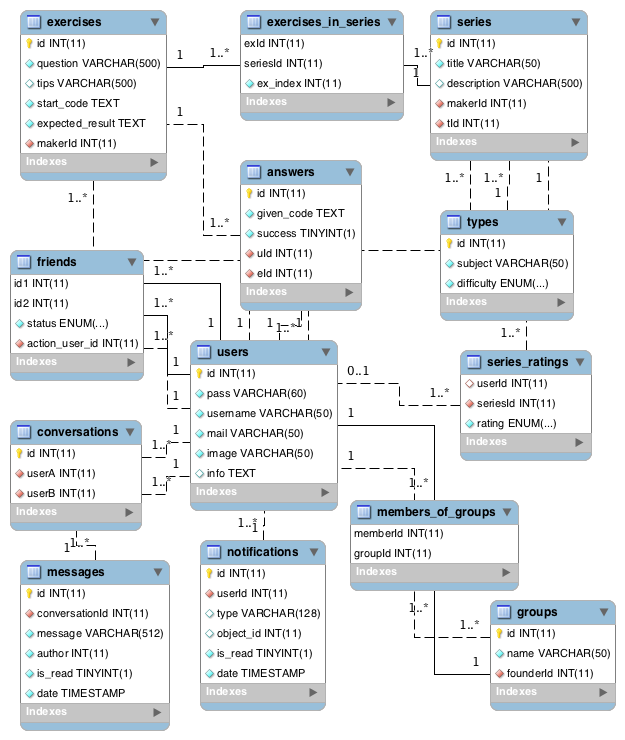
\includegraphics[keepaspectratio=true, scale=0.6]{raport_files/design/UML2.png}}\\
\small Hieronder wordt een korte uitleg gegeven over bovenstaande entiteiten. De uitbreiding van fase 2 t.o.v. fase 1
worden \textsl{licht cursief} weergegeven.
\normalsize
\begin{description}
    \item[Users] zijn de essentie van de website. Zij maken uit hoe succesvol de website kan zijn.
        Een User is 'een geregistreerd bezoeker'. \textsl{Users zijn uitgebreid om nu ook een afbeelding
        te bevatten, alsook een korte uitleg over de gebruiker. Beide zijn optionele attributen en mogen
        dus leeg blijven.}
    \item[Friends] is een 1-to-1 relatie. Om vrienden te worden moet een request verzonden worden.
        Indien de andere gebruiker dit aanvaard, is de Friends-relatie gecre\"{e}erd.
    \item[Groups] zijn verzamelingen van Users. Een groep wordt opgericht door een gebuiker, de 'founder'
        van de groep. Meerdere Users kunnen dan zonder meer lid worden van de groep. De gebruikers kunnen
        nadien de groep verlaten (met uitzondering van de 'founder'). Dit maakt dat een groep altijd minstens
        1 lid heeft.
    \item[Members of groups] zijn de gebruikers die lid zijn van een groep.
    \item[Converstations] zijn verzamelingen van berichten die tussen 2 gebruikers heen en weer gestuurd
        werden.
    \item[Messages] zijn de enkelvoudige berichten die van 1 gebruiker naar de andere gestuurd wordt.
        Alle messages van de ene gebruiker naar de andere en eventuele antwoorden vormen samen een conversation.
        \textsl{Een zeer kleine uitbreiding hierop is een controle of een bericht al dan niet gelezen is. Hierdoor
        kan de zender zien of zijn bericht aangekomen/gelezen is.}
    \item[Series] zijn het tweede essentiele deel van de applicatie. Een serie bestaat uit een set
        van 'Exercises'. Iedere serie krijgt ook een type en een rating.
    \item[Series rating] zijn de ratings die gebruikers aan een serie kunnen geven. Deze rating
        zal gebruikt worden om voorstellen te doen aan andere gebruikers.
    \item[Types] zijn tuples van een onderwerp en een moeilijkheidsgraad. Deze tuple vormt een
        unieke key van het type.
    \item[Exercises] vormen samen een serie. Iedere exercise bevat een vraag, (optionele) tips voor
        het oplossen van de oefening, start code die de gebruiker een beginpunt geeft en een verwacht resultaat.
        Dit verwacht resultaat wordt vergeleken met de gegenereerde output van de interpreter. \textsl{Exercises
        zijn niet langer verbonden aan een enkele serie. Om dit mogelijk te maken is een extra relatie toegevoegd:
        exercises\_in\_series. Een bijkomende uitbreiding is de mogelijkheid om als verwacht antwoord een reguliere
        expressie te geven. Deze wordt dan gematched met de gegenereerde oplossing.}
    \item[\textsl{Exercises\_in\_series}] \textsl{is een relatie tussen oefeningen en series. Hierin wordt gespecifieerd welke oefening
        in welke serie staat. Als bijkomend attribuut wordt de index van de oefening binnen de serie gespecifieerd.
        Hierdoor wordt de volgorde van oefeningen gecontroleerd. De beperking is opgesteld dat iedere oefening slechts 1x
        in een serie mag staan.}
    \item[Answers] zijn niet meer dan de aangepaste start code, samen met het resultaat
        van de interpreter. Zo kan een gebruiker de code later opnieuw opvragen en kan tegelijk snel
        opgevraagd worden of een gebruiker de oefening correct had opgelost.
    \item[\textsl{Notifications}] \textsl{zijn meldingen die een gebruiker kan krijgen. Denk hierbij aan bijvoorbeeld een
        ontvangen vriendschapsverzoek.}
\end{description}
